\selectlanguage{italian}
\graphicspath{ {img/1/} }
\chapter{Concetti di Biometria e Obiettivi}\label{cap:biometria}
\thispagestyle{empty} %Elimina il numero della prima pagina del capitolo.
\newpage
\section{Concetti di Biometria}
\vspace{8mm}
Le fasi di riconoscimento dell'iride disturbata sono gli stessi utilizzati in condizioni controllate, e quindi in sistemi "tradizionali", anche se richiedono approcci diversi a causa di caratteristiche dell'immagine quali la distanza dell'individuo dal dispositivo di cattura, la qualità dell'immagine e così via.\\
Tali fasi sono, in sequenza: acquisizione, segmentazione, normalizzazione, codifica, corrispondenza.

\begin{itemize}
    \item \textbf{Acquisizione}: rispetto ai sistemi tradizionali l'acquisizione non è necessariamente eseguita con dispositivi dedicati o videocamere di alta qualità. Immagini dell'iride possono essere ottenute da fotocamere semplici o attrezzature di acquisizione standard incorporate nel computer o dispositivi mobili. Le condizioni di acquisizione (illuminazione, distanza, posa, ecc) non sono strettamente controllate, contrariamente ai sistemi tradizionali.
    \item  \textbf{Segmentazione}: è il processo di identificazione dei confini dell'iride al fine di estrarre solo le informazioni dell'iride dalle immagini dell'occhio. Nei sistemi tradizionali, si tratta di un'operazione relativamente semplice che consiste nel trovare due cerchi che corrispondono con i bordi pupilla-iride e pupilla-sclera.
    Nell'iride disturbata il processo di segmentazione è molto più complicato. Si deve tener conto dell’eventuale presenza di occlusioni o riflessi, che devono essere scartati, nel senso che la superficie corrispondente non deve essere considerata per la codifica e il confronto. L'individuazione dei confini è ulteriormente ostacolata dalla bassa risoluzione o presenza di rumore, che rendono i confini meno chiari. Per questo motivo i metodi di segmentazione dell'iride disturbata di solito implementano una fase di pre-elaborazione in cui vengono applicati filtri di smoothing (per ridurre il rumore) e/o filtri di miglioramento (per migliorare le caratteristiche, come i confini dell'iride)
    \item \textbf{Normalizzazione}: nei sistemi tradizionali, a causa della condizione di acquisizione controllata, è necessario solo normalizzare la forma segmentata dell'iride. La normalizzazione tipica implica la trasformazione di coordinate cartesiane in quelle polari. Se si tiene conto delle informazioni sul colore, correzione del colore, istogramma di normalizzazione o operazioni simili possono essere risultare utili.
    \item \textbf{Codifica}: questa fase produce un vettore modello di caratteristiche, cioè una rappresentazione compatta di un'immagine dell'iride. Le differenze negli algoritmi di estrazione di caratteristiche quando le iridi disturbate vengono processate dipendono dal fatto che in immagini di alta qualità anche piccoli dettagli strutturali dell'iride sono facilmente visibili. Al contrario, le immagini disturbate possono presentare caratteristiche alterate o meno caratteristiche da osservare. Approcci per l'estrazione di caratteristiche di immagini disturbate analizzano principalmente la texture dell'iride, quali la distribuzione del colore, la presenza di regioni più chiare o più scure e possono combinare un certo numero di operatori, ognuno applicato a una particolare caratteristica
     \item \textbf{Corrispondenza}: la fase di confronto dipende solo dal tipo di modelli utilizzati.\cite{biometria}\newpage
\end{itemize}

\begin{figure}[h!]
	\centering
	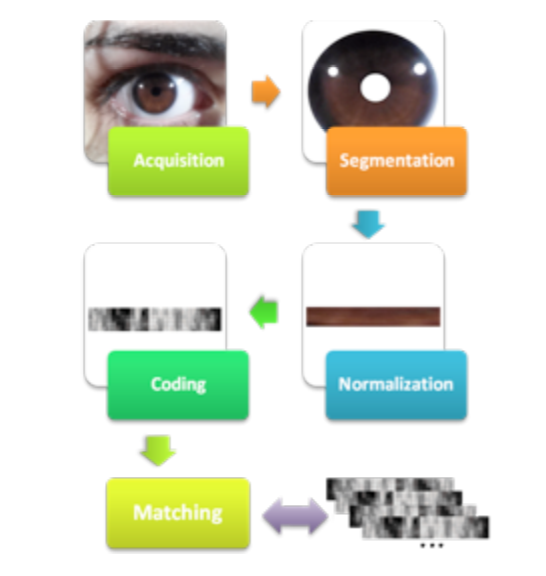
\includegraphics[width=90mm]{img/1/bio_1_1.PNG}
	\caption{\fontsize{10px}{0mm}\selectfont Sequenza delle fasi utili al riconoscimento dell'iride \label{fig:bio_1_1}}
\end{figure}
\section{Obiettivi}
\vspace{8mm}
Gli obiettivi sono quindi la realizzazione di metodologie per effettuare acquisizione, segmentazione, normalizzazione e coding dell'iride in contesti non controllati, in particolare, esse saranno implementate utilizzando un dispositivo comune quale la webcam.
Le metodologie in questione faranno parte di un sistema in grado di utilizzare le metodologie precedenti e capace quindi di ottenere, in particolare, riconoscimento, segmentazione e coding dell'iride.\newpage